% XeLaTeX

\documentclass{article}
\usepackage{ctex}
\usepackage{xypic}
\usepackage{amsfonts,amssymb}
\usepackage{multirow}
\usepackage{geometry}
\usepackage{graphicx}
\usepackage{listings}
\usepackage{lipsum}
\usepackage{courier}
\usepackage{fancyvrb}
\usepackage{etoolbox}
\usepackage{nameref}
\usepackage[titletoc]{appendix}

\usepackage{tikz}
\usetikzlibrary{calc,trees,positioning,arrows,chains,shapes.geometric,
decorations.pathreplacing,decorations.pathmorphing,shapes,
matrix,shapes.symbols}
\usepackage[european]{circuitikz}

\linespread{1.2}
\geometry{left=3cm,right=2.5cm,top=2.5cm,bottom=2.5cm}

\makeatletter
\patchcmd{\FV@SetupFont}
  {\FV@BaseLineStretch}
  {\fontencoding{T1}\FV@BaseLineStretch}
  {}{}
\makeatother

\lstset{basicstyle=\small\fontencoding{T1}\ttfamily,breaklines=true}
\lstset{numbers=left,frame=shadowbox,tabsize=4}
%\lstset{extendedchars=false}
\begin{document}

\title{中断控制器的设计与实现}
\author {王凯祺\ \ \ \ 16337233 \\
数据科学与计算机学院 \ \ \ \ 2016级计算机类教务3班 \\
指导老师:李国桢
}
\maketitle

\tableofcontents

\newpage

\section{选题背景}

在《计算机组成原理》课程中,我学习到了单周期 CPU 、多周期 CPU 和流水线 CPU 的工作原理。通过实验,我更加清楚地了解了 CPU 取指令、指令译码、指令执行、存储器访问、结果写回这 5 个阶段。本学期在以 Computer Organization and Design \cite{COD} 为课本的学习过程中,本书在第 4.9 节为我介绍了系统中断,并提供了处理异常的数据通路。但是书上并没有介绍中断程序计数器(EPC)是如何工作的,也没有告诉我如果加上处理异常的功能,CPU 的控制单元需要做哪些改变。由于此部分没有更详尽的文档,我们在实验课上就没有做异常处理的内容。我希望自己设计一个中断控制器,与我先前设计的多周期 CPU 合并成一块可以处理中断的多周期CPU ,为之后做此项实验的同学提供一份较为详细的设计过程供参考。

\section{技术路线}

我选择赛灵思(Xilinx)Vivado 设计套件作为设计、编译和仿真软件。在器件设计上,我使用 Verilog HDL 设计中断控制器、中断向量表存储器以及中断堆栈。在实验课上,我已实现了不含中断控制器的 CPU 。为了测试我的中断控制器,我将该 CPU 稍加修改,加入中断周期,再连接我自主设计的中断控制器,变成可处理中断的 CPU ,就可以对中断控制器进行测试了。

\section{设计过程}

\subsection{中断处理流程}

CPU 完成中断响应动作后,首先保存当前断点、关总中断,然后查询中断向量表,并取出中断向量地址并跳转。最后还原现场,返回原断点 \cite{ARM} 。

该过程示意图如图 \ref{M1} 所示。

\tikzset{
>=stealth',
  punktchain/.style={
    rectangle, 
    rounded corners, 
    % fill=black!10,
    draw=black, very thick,
    text width=10em, 
    minimum height=3em, 
    text centered, 
    on chain},
  line/.style={draw, thick, <-},
  element/.style={
    tape,
    top color=white,
    bottom color=blue!50!black!60!,
    minimum width=8em,
    draw=blue!40!black!90, very thick,
    text width=10em, 
    minimum height=3.5em, 
    text centered, 
    on chain},
  coord/.style={coordinate, on chain, on grid, node distance=6mm and 25mm},
  every join/.style={->, thick,shorten >=1pt},
  decoration={brace},
  tuborg/.style={decorate},
  tubnode/.style={midway, right=2pt},
}

\begin{figure}[!h]
\centering

\begin{tikzpicture}
	[node distance=.8cm,
	start chain=going below,]
	\node[punktchain, join] (p0) {中断发生};
	\node[punktchain, join] (p1) {保存程序断点};
	\node[punktchain, join] (p2) {关总中断};
	\node[coord, join, right=of p2] (c2) {};
	\node[coord, join, right=of p0] (c0) {};
	\node[punktchain, join, right=of c0] (p3) {查找中断源};
	\node[punktchain, join] (p4) {中断判优};
	\node[punktchain, join] (p5) {查找动态中断向量表};
	\node[coord, join, right=of p5] (c5) {};
	\node[coord, join, right=of p3] (c3) {};
	\node[punktchain, join, right=of c3] (p6) {取出中断服务程序执行};
	\node[punktchain, join] (p7) {执行中断服务程序};
	\node[punktchain, join] (p8) {中断返回};
\end{tikzpicture}
\caption{中断处理流程示意图}
\label{M1}
\end{figure}


\subsection{中断控制器设计}

\def\intSwitch(#1)#2{
	\begin{scope}[shift={(#1)}]
		\draw (0,0) rectangle (5,2);
		\draw (2.5,2) -- (2.5,0);
		\node at (3.75,1) {intSwitchOut};
		\draw (5,1) -- +(0.25,0) coordinate(#2 intSwitchOut);
		\draw (0,0.4) node[right] {intSwitchIn} -- + (-0.25,0) coordinate (#2 intSwitchIn);
		\draw (0,1.0) node[right] {Enable} -- + (-0.25,0) coordinate (#2 Enable);
		\draw (0,1.6) node[right] {clk} -- + (-0.25,0) coordinate (#2 clk);
		\node at (2.5,-0.25) {中断允许标志};
	\end{scope}
}

\def\intControl(#1)#2{
	\begin{scope}[shift={(#1)}]
		\draw (0,0) rectangle (5,2);
		\draw (2.5,2) -- (2.5,0);
		\node at (3.75,1.6) {intWre};
		\node at (3.75,1.0) {intEntryAddr};
		\node at (3.75,0.4) {Hardint};
		\draw (5,1.6) -- +(0.25,0) coordinate (#2 intWre);
		\draw (5,1.0) -- +(0.25,0) coordinate (#2 intEntryAddr);
		\draw (5,0.4) -- +(0.25,0) coordinate (#2 Hardint);
		\draw (0,1.75) node[right] {intSwitch} -- + (-0.25,0) coordinate (#2 intSwitch);
		\draw (0,1.25) node[right] {HardintInput} -- + (-0.25,0) coordinate (#2 HardintInput);
		\draw (0,0.75) node[right] {SoftintInput} -- + (-0.25,0) coordinate (#2 SoftintInput);
		\draw (0,0.25) node[right] {SoftintWre} -- + (-0.25,0) coordinate (#2 SoftintWre);
		\node at (2.5,-0.25) {中断判优逻辑};
	\end{scope}
}

\def\intVectorROM(#1)#2{
	\begin{scope}[shift={(#1)}]
		\draw (0,0) rectangle(5,0.5);
		\draw (2.5,0.5) -- (2.5,0);
		\node at (3.75,0.25) {intVectorAddr};
		\draw (5,0.25) -- +(0.25,0) coordinate (#2 intVectorAddr);
		\draw (0,0.25) node[right] {intEntryAddr} -- + (-0.25,0) coordinate (#2 intEntryAddr);
		\node at (2.5,-0.25) {中断向量表存储器};
	\end{scope}
}

\begin{figure}
\centering

\begin{tikzpicture}[every path/.style={},>=triangle 45]
	\intSwitch(0,0){a}
	\intControl(7,0){b}
	\intVectorROM(7,-2){c}
	\draw (a intSwitchOut) |- (b intSwitch);
	\draw (13,-1) -- +(0,0) coordinate(d);
	\draw (6,-1) -- +(0,0) coordinate(e);
	\draw (d) -- (e);
	\draw (e) |- (c intEntryAddr);
	\draw (b intEntryAddr) -| (d);
\end{tikzpicture}
\caption{中断控制器元器件及连线图}
\label{M2}
\end{figure}

中断控制器是一个中断判优的组合电路,根据输入的中断源,选择优先级最高的响应,并把对应的中断入口地址接到中断向量表存储器中,由中断向量表存储器查询中断向量地址,接到PC输入端。

中断控制器元器件及连线图如图 \ref{M2} 所示。

\paragraph{中断允许标志}

中断允许标志用于允许或禁止响应中断。 CPU 在响应中断期间,须将中断允许标志清零,即CPU处于禁止中断状态。进入中断服务程序后,须将中断允许标志置 1 ,开放中断。\cite{COD2}

中断允许标志使用了一个带使能端的 D 触发器,其使能端和数据输入端接 CPU ,由 CPU 控制中断允许标志是否置 1 。中断允许标志的输出接到中断判优逻辑。

\paragraph{中断判优逻辑}

中断判优逻辑共有 4 个输入端,和 3 个输出端。

输入 intSwitch 表示中断允许标志,接中断允许标志的输出;

输入 HardintInput 表示硬中断的输入信号;

输入 SoftintInput 表示软中断的输入信号,接指令中的立即数;

输入 SoftintWre 表示软中断使能端,接 CPU;

输出 intWre 表示是否响应中断,接 CPU;

输出 intEntryAddr 表示中断入口地址,接中断向量表存储器;

输出 Hardint 表示系统响应的是否为硬中断(高电平表示是)。

若中断关闭,则不响应中断;若中断打开,选择最高优先级的中断源响应,并将中断入口地址输出。

在一个计算机系统中,存在多个中断源。中断优先级根据各个中断事件的轻重缓急程度的不同分成若干级别,给每个中断源分配一个优先权。中断判优有两种实现方法:硬件电路法和软件查询法 \cite{COD2} 。为了让电路简单,我使用软件查询法来判断中断优先级。

软件查询法的流程图如图 \ref{M3} 所示 \cite{COD2} 。

\tikzset{
  base/.style={draw, on chain, on grid, align=center, minimum height=4ex},
  proc/.style={base, rectangle, text width=8em},
  test/.style={base, diamond, aspect=2, text width=5em},
  term/.style={proc, rounded corners},
  null/.style={base, draw=none, fill=none},
  % coord node style is used for placing corners of connecting lines
  coord/.style={coordinate, on chain, on grid, node distance=6mm and 25mm},
  % nmark node style is used for coordinate debugging marks
  nmark/.style={draw, cyan, circle, font={\sffamily\bfseries}},
  % -------------------------------------------------
  % Connector line styles for different parts of the diagram
  norm/.style={->, draw},
  free/.style={->, draw},
  cong/.style={->, draw},
  it/.style={font={\small\itshape}}
}

\begin{figure}
\centering
\begin{tikzpicture}[%
    >=triangle 60,              % Nice arrows; your taste may be different
    start chain=going below,    % General flow is top-to-bottom
    node distance=6mm and 60mm, % Global setup of box spacing
    every join/.style={norm},   % Default linetype for connecting boxes
    ]
    \node [proc] (p0) {开始};
    \node [test, join] (p1) {有 1 号中断请求?};
    \node [test] (p2) {有 2 号中断请求?};
    \node [null] (ps) {$\vdots$};
    \node [test] (p3) {有 n 号中断请求?};
    \node [proc] (p4) {中断返回};
    \node [proc, right=of p1] (q1) {执行 1 号中断服务程序};
    \node [proc, right=of p2] (q2) {执行 2 号中断服务程序};
    \node [null, right=of ps] (qs) {$\vdots$};
    \node [proc, right=of p3] (q3) {执行 n 号中断服务程序};
    \node [null, right=of q1] (r1) {};
    \node [null, right=of q2] (r2) {};
    \node [null, right=of qs] (rs) {};
    \node [null, right=of q3] (r3) {};
    \path (p1.south) to node [xshift=1em] {否} (p2);
    	\draw [->] (p1.south) -- (p2);
    \path (p2.south) to node [xshift=1em] {否} (ps);
    	\draw [->] (p2.south) -- (ps);
    \path (ps.south) to node [xshift=1em] {否} (p3);
    	\draw [->] (ps.south) -- (p3);
    \path (p3.south) to node [xshift=1em] {否} (p4);
    	\draw [->] (p3.south) -- (p4);
	\draw (q1.east) -| (r1.south);
	\draw (q2.east) -| (r2.south);
	\draw (q3.east) -| (r3.south);
    \draw [->] (r1.south) |- (p4);
    \path (p1.east) to node [yshift=1em] {是} (q1);
    	\draw [->] (p1.east) -- (q1);
    \path (p2.east) to node [yshift=1em] {是} (q2);
    	\draw [->] (p2.east) -- (q2);
    \path (p3.east) to node [yshift=1em] {是} (q3);
    	\draw [->] (p3.east) -- (q3);
    
    
\end{tikzpicture}    

\caption{软件查询法流程图}
\label{M3}

\end{figure}

\subsection{堆栈设计}

中断服务程序结束后,必须能正确地返回到被中断的断点处继续原来程序的执行。为了保存断点位置,同时为了支持中断嵌套,我们需要实现一个硬件堆栈。

硬件堆栈用计数器记录栈顶位置,用存储器保存堆栈中元素的值。我们可以把它们写成一个模块,如图 \ref{M4} 。

在图 \ref{M4} 中,pushWre 表示压栈操作使能端,popWre 表示弹出操作使能端,StackTop 表示当前堆栈中实时的栈顶元素。由于弹出元素的操作会使 StackTop 立即发生改变,我们增加 D 触发器延迟该改变,保证在弹出元素的过程中仍然可以访问栈顶元素的值。


\def\Stack(#1)#2{
	\begin{scope}[shift={(#1)}]
		\draw (0,0) rectangle(5,2);
		\draw (2.5,2) -- (2.5,0);
		\node at (3.75,1.0) {StackTop};
		\draw (5,1.0) -- +(0.25,0) coordinate (#2 StackTop);
		\draw (0,1.75) node[right] {clk} -- + (-0.25,0) coordinate (#2 clk);
		\draw (0,1.25) node[right] {pushWre} -- + (-0.25,0) coordinate (#2 pushWre);
		\draw (0,0.75) node[right] {popWre} -- + (-0.25,0) coordinate (#2 popWre);
		\draw (0,0.25) node[right] {dataIn} -- + (-0.25,0) coordinate (#2 dataIn);
	\end{scope}
}

\def\DTrigger(#1)#2{
	\begin{scope}[shift={(#1)}]
		\draw (0,0) rectangle(2,1);
		\draw (1,1) -- (1,0);
		\node at (1.5,0.5) {Q};
		\draw (2,0.5) -- + (0.25,0) coordinate (#2 Q);
		\draw (0,0.75) node[right] {clk} -- + (-0.25,0) coordinate (#2 clk);
		\draw (0,0.25) node[right] {D} -- + (-0.25,0) coordinate (#2 D);
	\end{scope}
}

\begin{figure}
\centering

\begin{tikzpicture}[every path/.style={},>=triangle 45]
	\Stack(0,0){a}
	\DTrigger (7,0.75) {b}
	\draw (a StackTop) -- (b D);
	\draw (b clk) -- (6,1.5);
	\draw (6,1.5) -- (6,3);
	\draw (6,3) -- (-2,3);
	\draw (-1,3) -- (-1,1.75);
	\draw (-1,1.75) -- (a clk);
\end{tikzpicture}
\caption{硬件堆栈设计图}
\label{M4}
\end{figure}

\subsection{中断指令设计}

我根据 MIPS 的指令集,设计了 3 条中断指令用于测试中断控制器。

\subsubsection{软中断指令}

功能:系统中断调用,中断入口地址为 immediate 。执行该指令时,同时关闭系统中断,将PC+4压入堆栈,并将PC转移到中断向量地址。

类型: I类型

用法: int \emph{immediate}

机器码:

\begin{table}[!hbp]
	\begin{tabular}{|l|l|l|l|}
		\hline
		操作码 & RS & RT & 立即数 \\
		\hline
		101001 & 00000(未用) & 00000(未用) & immediate(16位)\\
		\hline
	\end{tabular}
\end{table}

\subsubsection{开放中断指令}

功能:限中断服务程序使用,用于打开系统中断。中断控制器不再屏蔽可屏蔽中断。

类型: J类型

用法: yes

机器码:

\begin{table}[!hbp]
	\begin{tabular}{|l|l|l|l|}
		\hline
		操作码 & \\
		\hline
		101000 & 00000000000000000000000000\\
		\hline
	\end{tabular}
\end{table}

\subsubsection{中断返回指令}

功能:限中断服务程序使用,返回到断点地址。执行该指令时,同时打开系统中断,转移到栈顶地址,并弹出堆栈。

类型: J类型

用法: ret

机器码:

\begin{table}[!hbp]
	\begin{tabular}{|l|l|l|l|}
		\hline
		操作码 & \\
		\hline
		101010 & 00000000000000000000000000\\
		\hline
	\end{tabular}
\end{table}

\subsection{重新设计 CPU 状态}

为了测试中断控制器,我们还需要修改多周期 CPU ,使该 CPU 可以处理中断。

\subsubsection{不含中断控制器的多周期 CPU}

不含中断控制器的多周期CPU状态转移图如图 \ref{M5} 所示。\textbf{本部分内容为实验课内容}。

不含中断控制器的多周期 CPU 在处理指令时,一般需要经过以下几个阶段:

1. 取指令(IF):根据程序计数器 PC 中的指令地址,从存储器中取出一条指令,送入指令寄存器中。

2. 指令译码(ID):对取指令操作中得到的指令进行分析并译码,确定这条指令需要完成的操作,从而产生相应的操作控制信号,用于驱动执行状态中的各种操作。

3. 指令执行(EXE):根据指令译码得到的操作控制信号,具体地执行指令动作,然后转移到结果写回状态。

4. 存储器访问(MEM):给定存储器的数据地址,把数据写入到存储器中数据地址所指定的存储单元或者从存储器中得到数据地址单元中的数据。

5. 结果写回(WB):指令执行的结果或者访问存储器中得到的数据写回相应的目的寄存器中。

\tikzset{
  base/.style={draw, on chain, on grid, align=center, minimum height=4ex},
  proc/.style={base, rectangle, text width=8em},
  test/.style={base, diamond, aspect=2, text width=5em},
  term/.style={proc, rounded corners},
  null/.style={base, draw=none, fill=none},
  % coord node style is used for placing corners of connecting lines
  coord/.style={coordinate, on chain, on grid, node distance=6mm and 25mm},
  % nmark node style is used for coordinate debugging marks
  nmark/.style={draw, cyan, circle, font={\sffamily\bfseries}},
  % -------------------------------------------------
  % Connector line styles for different parts of the diagram
  norm/.style={->, draw},
  free/.style={->, draw},
  cong/.style={->, draw},
  it/.style={font={\small\itshape}}
}

\begin{figure}
\centering
\begin{tikzpicture}[%
	->,
    >=triangle 60,              % Nice arrows; your taste may be different
    start chain=going below,    % General flow is top-to-bottom
    node distance=6mm and 60mm, % Global setup of box spacing
    every join/.style={norm},   % Default linetype for connecting boxes
    ]
    \node [proc] (sIF) {取指令 IF (000)};
    \node [proc, right=of sIF] (sID) {指令译码 ID (001)};
    \node [proc, right=of sID] (sEXE) {指令执行 EXE (010)};
    \node [proc, below=of sEXE, yshift=-9em] (sMEM) {存储器访问 MEM (011)};
    \node [proc, left=of sMEM] (sWB) {结果写回 WB (100)};
   	\path (sIF.east) edge [bend right=60] node {} (sID.west);
    \path (sID.east) to node [yshift=3em] {\shortstack[l]{add, sub, addi, \\ or, and, ori, \\ sll, slt, slti, \\ beq, bne, bgtz, \\ sw, lw}} (sEXE);
    	\draw [->] (sID.east) -- (sEXE);
    	
    \path (sID.west) edge[bend right=60] node {\shortstack[l]{j, jal, jr, halt}} (sIF.east);
    \path (sEXE.north) edge[ bend right=60 ] node {\shortstack[l]{beq, bne, bgtz}} (sIF.north);
    \path (sEXE.south) edge node {\shortstack[l]{sw, lw}} (sMEM.north);
    \path (sEXE.south) edge node {\shortstack[l]{add, sub, addi, \\ or, and, ori, \\ sll, slt, slti}} (sWB.north);
    \path (sMEM.west) edge node {\shortstack[l]{lw}} (sWB.east);
    \path (sMEM.west) edge [ bend left=60 ] node {\shortstack[l] {sw}} (sIF.south);
    \path (sWB.west) edge[ bend left=30 ] node {} (sIF.south);
\end{tikzpicture}    


\caption{不含中断控制器的多周期 CPU 状态转移图}
\label{M5}
\end{figure}

\subsubsection{含中断控制器的多周期 CPU}

含中断控制器的多周期CPU状态转移图如图 \ref{M6} 所示。图中下方的元件以及黑色和蓝色的线均为实验课上设计不含中断控制器的多周期CPU时\emph{何朝东老师}提供的,上方的元件及绿色的线是我画的。

含中断控制器的多周期CPU需要能同时处理软中断和硬中断,则需在原状态转移图的基础上加上一个中断周期。这个中断周期必须在指令译码前或者整条指令执行完毕后。如果不然,某些指令的执行过程中将不包含中断周期,执行那些指令时无法响应中断,这是我们不愿意看到的。所以我把中断周期放在取指令(IF)阶段和指令译码(ID)阶段之间。

指令的执行步骤:

1. 首先取指令到指令寄存器中。

2. 在中断周期,将硬中断、软中断信号传输给中断控制器,由中断控制器决定是否响应中断。

3. 若中断控制器决定响应中断,则将当前 PC (硬中断)或 PC + 4 (软中断)压入堆栈,查询中断向量地址并将PC转移到中断向量地址,回到取指令(IF)阶段;若中断控制器决定不予响应中断,则继续执行指令译码(ID)等步骤。

含中断控制器的多周期CPU数据通路图如图 \ref{M7} 所示。


\tikzset{
  base/.style={draw, on chain, on grid, align=center, minimum height=4ex},
  proc/.style={base, rectangle, text width=8em},
  test/.style={base, diamond, aspect=2, text width=5em},
  term/.style={proc, rounded corners},
  null/.style={base, draw=none, fill=none},
  % coord node style is used for placing corners of connecting lines
  coord/.style={coordinate, on chain, on grid, node distance=6mm and 25mm},
  % nmark node style is used for coordinate debugging marks
  nmark/.style={draw, cyan, circle, font={\sffamily\bfseries}},
  % -------------------------------------------------
  % Connector line styles for different parts of the diagram
  norm/.style={->, draw},
  free/.style={->, draw},
  cong/.style={->, draw},
  it/.style={font={\small\itshape}}
}

\begin{figure}
\centering
\begin{tikzpicture}[%
	->,
    >=triangle 60,              % Nice arrows; your taste may be different
    start chain=going below,    % General flow is top-to-bottom
    node distance=6mm and 60mm, % Global setup of box spacing
    every join/.style={norm},   % Default linetype for connecting boxes
    ]
    \node [proc] (sIF) {取指令 IF (000)};
    \node [proc, right=of sIF] (sID) {指令译码 ID (001)};
    \node [proc, right=of sID] (sEXE) {指令执行 EXE (010)};
    \node [proc, below=of sEXE, yshift=-9em] (sMEM) {存储器访问 MEM (011)};
    \node [proc, left=of sMEM] (sWB) {结果写回 WB (100)};
    \node [proc, left=of sWB] (sINT) {中断周期 INT (101)};
   	\path (sIF.south) edge node {} (sINT.north);
   	\path (sINT.west) edge [bend left=45] node {响应中断} (sIF.west);
   	\path (sINT.north) edge node {不予响应中断} (sID.south);
    \path (sID.east) to node [yshift=3em] {\shortstack[l]{add, sub, addi, \\ or, and, ori, \\ sll, slt, slti, \\ beq, bne, bgtz, \\ sw, lw}} (sEXE);
    	\draw [->] (sID.east) -- (sEXE);
    	
    \path (sID.west) edge node {\shortstack[l]{j, jal, jr, halt}} (sIF.east);
    \path (sEXE.north) edge[ bend right=60 ] node {\shortstack[l]{beq, bne, bgtz}} (sIF.north);
    \path (sEXE.south) edge node {\shortstack[l]{sw, lw}} (sMEM.north);
    \path (sEXE.south) edge node {\shortstack[l]{add, sub, addi, \\ or, and, ori, \\ sll, slt, slti}} (sWB.north);
    \path (sMEM.west) edge node {\shortstack[l]{lw}} (sWB.east);
%    \path (sMEM.west) edge node {\shortstack[l] {sw}} (sIF.east);
	\path (sMEM.west) edge [ bend left=60 ] node {\shortstack[l] {sw}} (sIF.south);
    \path (sWB.west) edge[ bend left=30 ] node {} (sIF.south);
\end{tikzpicture}    


\caption{含中断控制器的多周期 CPU 状态转移图}
\label{M6}
\end{figure}

\begin{figure}
\centering
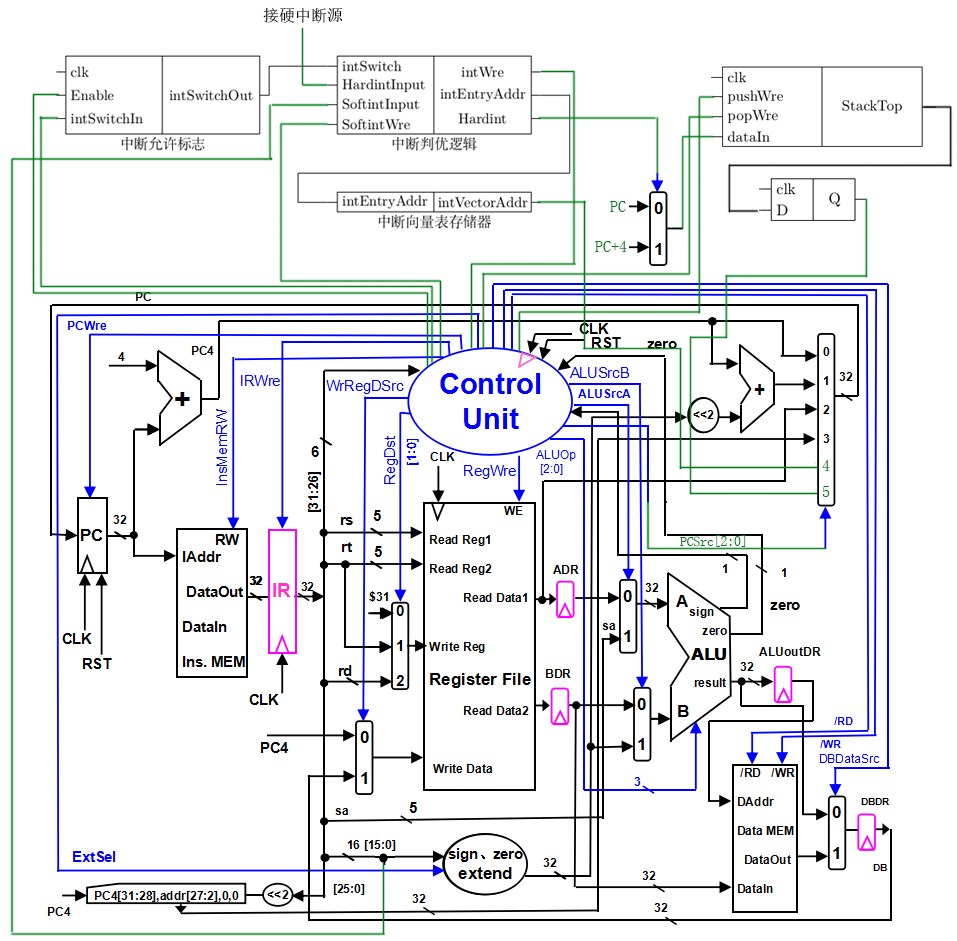
\includegraphics[scale=0.65]{../pics/DataPath.png}
\caption{含中断控制器的多周期 CPU 数据通路图}
\label{M7}
\end{figure}

\subsection{模拟仿真}

\subsubsection{测试程序段}

我设计了一串指令序列用于测试 CPU 及中断控制器。硬中断通过开关输入中断控制器,软中断通过 int 指令输入 CPU 。

测试程序段如表 \ref{T1} 。

中断向量表如表 \ref{T2} 。

\begin{table}[!h]
\centering
\begin{tabular}{|l|l|l|l|l|l|}
\hline
地址 & 汇编程序 & op(6) & rs(5) & rt(5) & rd(5) / immediate(16) \\
\hline
0x00000000 & addi \$1, \$0, 8 & 000010 & 00000 & 00001 & 0000 0000 0000 1000 \\
\hline
0x00000004 & ori \$2, \$0, 2 & 010010 & 00000 & 00010 & 0000 0000 0000 0010 \\
\hline
0x00000008 & or \$3, \$2, \$1 & 010000 & 00010 & 00001 & 0001 1000 0000 0000 \\
\hline
0x0000000C & sub \$4, \$3, \$1 & 000001 & 00011 & 00001 & 0010 0000 0000 0000 \\
\hline
0x00000010 & or \$5, \$4, \$2 & 010000 & 00100 & 00010 & 0010 1000 0000 0000 \\
\hline
0x00000014 & int 2 & 101001 & 00000 & 00000 & 0000 0000 0000 0010 \\
\hline
0x00000018 & addi \$1, \$1, 2 & 000010 & 00001 & 00001 & 0000 0000 0000 0000 \\
\hline
0x0000001C & halt & 111111 & 00000 & 00000 & 0000 0000 0000 0000 \\
\hline
0x00000020 & & 000000 & 00000 & 00000 & 0000 0000 0000 0000 \\
\hline
0x00000024 & yes & 101000 & 00000 & 00000 & 0000 0000 0000 0000 \\
\hline
0x00000028 & addi \$1, \$1, 1 & 000010 & 00001 & 00001 & 0000 0000 0000 0001 \\
\hline
0x0000002C & ret & 101010 & 00000 & 00000 & 0000 0000 0000 0000 \\
\hline
0x00000030 & & 000000 & 00000 & 00000 & 0000 0000 0000 0000 \\
\hline
0x00000034 & addi \$1, \$1, 2 & 000010 & 00001 & 00001 & 0000 0000 0000 0010 \\
\hline
0x00000038 & ret & 101010 & 00000 & 00000 & 0000 0000 0000 0000 \\
\hline
0x0000003C & & 000000 & 00000 & 00000 & 0000 0000 0000 0000 \\
\hline
0x00000040 & yes & 101000 & 00000 & 00000 & 0000 0000 0000 0000 \\
\hline
0x00000044 & addi \$1, \$1, 3 & 000010 & 00001 & 00001 & 0000 0000 0000 0011 \\
\hline
0x00000048 & ret & 101010 & 00000 & 00000 & 0000 0000 0000 0000 \\
\hline

\end{tabular}
\caption{测试程序段}
\label{T1}
\end{table}

\begin{table}[!h]
\centering
\begin{tabular}{|l|l|}
\hline
中断入口地址 & 中断向量地址 \\
\hline
0x00 & 0x00000024 \\
\hline
0x01 & 0x00000034 \\
\hline
0x02 & 0x00000040 \\
\hline
\end{tabular}
\caption{中断向量表}
\label{T2}
\end{table}

\subsubsection{时序仿真}

测试程序段初始化在指令存储器中,中断向量表初始化在中断向量表存储器中。

时钟周期为 40 ns 。

在仿真过程中,200 ns - 300 ns 同时出现 0 号硬中断和 1 号硬中断; 460 ns - 580 ns 出现 1 号硬中断。

时序仿真波形图如图 \ref{B1} 所示。由于版面所限,未能将完整的波形图放在正文部分。请参照附录以查看完整波形图。

\begin{figure}
\centering
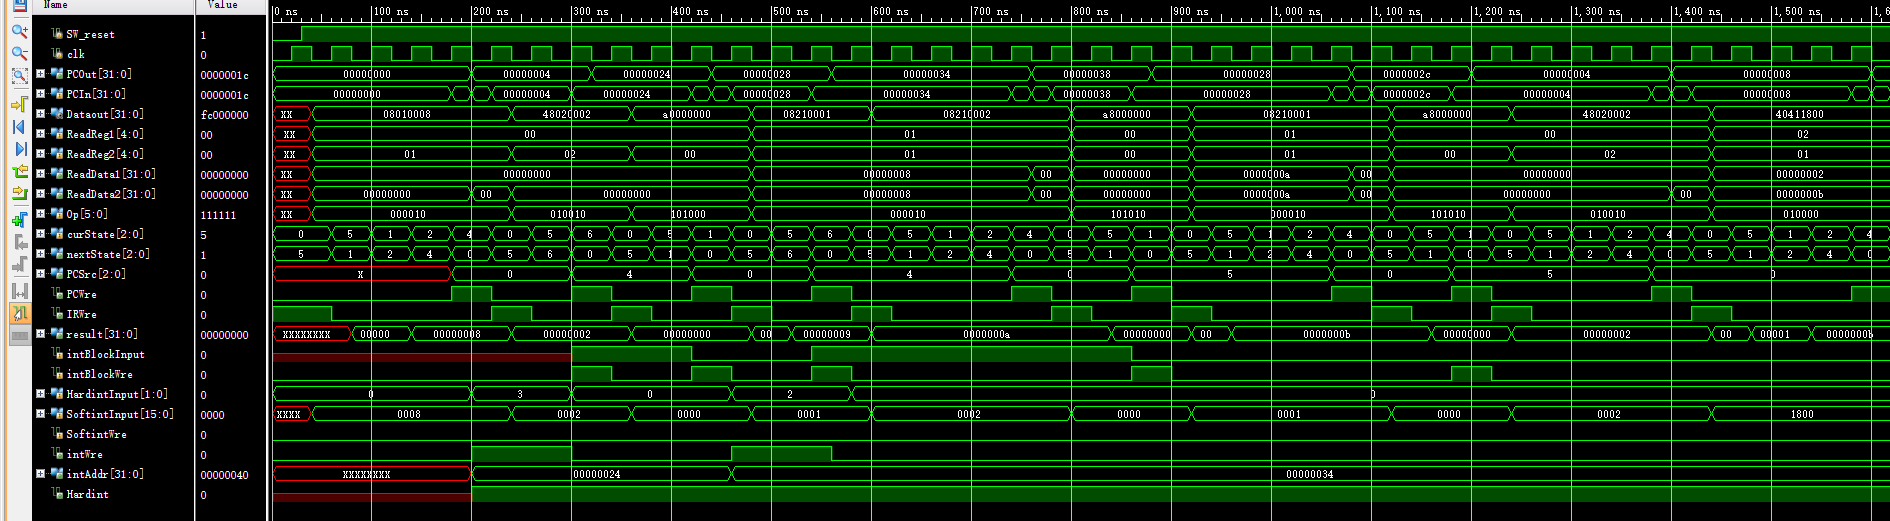
\includegraphics[scale=0.24]{../pics/img_full_1.png}
\caption{时序仿真波形图}
\label{B1}
\end{figure}

通过波形图,我们可以看到该 CPU 和中断控制器能正常工作,可以同时处理软中断以及硬中断,可以处理中断嵌套的情况,可以处理多中断判优的情况。

\section{效果评价}

我设计的中断控制器能处理软硬中断,可以处理中断嵌套和多中断判优的情况。由于时间有限,没有来得及写输入、输出以及其它中断的中断服务程序,只提供了一段示例中断服务程序用于测试中断控制器,但在我设计的中断控制器及CPU上,可以在开发了输入、输出等中断服务程序的情况下处理输入、输出等中断。

自己设计一个中断控制器相比于设计 CPU 来说简单一些,但仍是一个复杂且耗时的过程,这同样需要严谨的思考和仔细的设计。在设计的过程中,我也遇到了不少的困难。由于 CPU 的控制器与中断判优逻辑均为组合电路,CPU 修改中断允许标志(intSwitchIn = 0)后,在下降沿会立即收到中断判优逻辑不予响应中断(intWre = 0)的信号,导致 CPU 控制器输出错误的指令。考虑到单个周期会产生冲突,我将中断周期拆成两个周期去完成,第一个周期先判优,将是否响应中断的结果先通过一个 D 触发器,然后给 CPU 控制器;第二个周期修改中断允许标志就不会出错了。

我的中断控制器仅在中断处理流程参考了《高校教材 \ 计算机组成原理》 \cite{COD2} ,其余部分均为自主设计的。这个中断控制器填补了课本上在中断控制方面的空白。希望我设计的中断控制器可供以后学习《计算机组成原理》这门课程的同学参考。

\renewcommand\refname{参考文献}
\bibliographystyle{plain}
\bibliography{report}

\newpage
\appendix
\appendixpage
\addcontentsline{toc}{section}{附录}\markboth{APPENDICES}{}
\begin{appendices}
\section{时序仿真波形图}

\begin{figure}[!h]
\centering
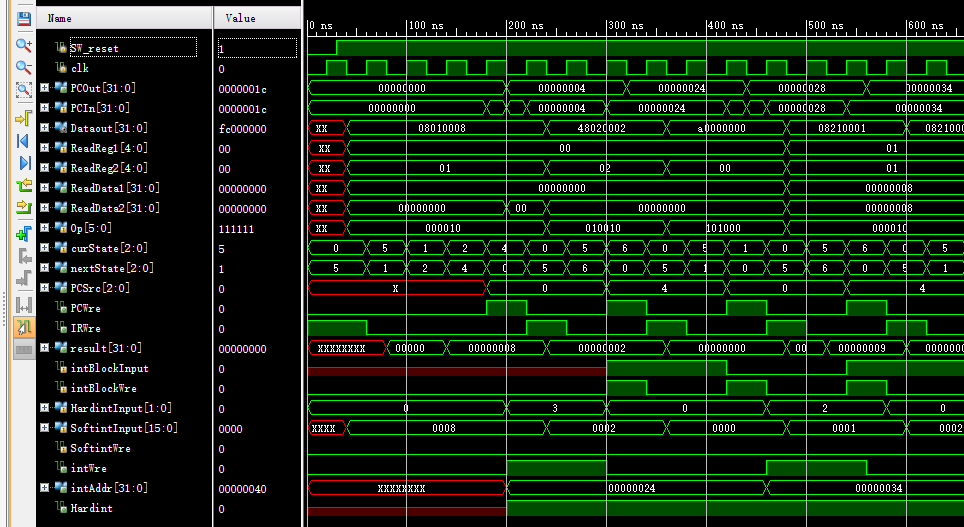
\includegraphics[scale=0.45]{../pics/img_1.png}
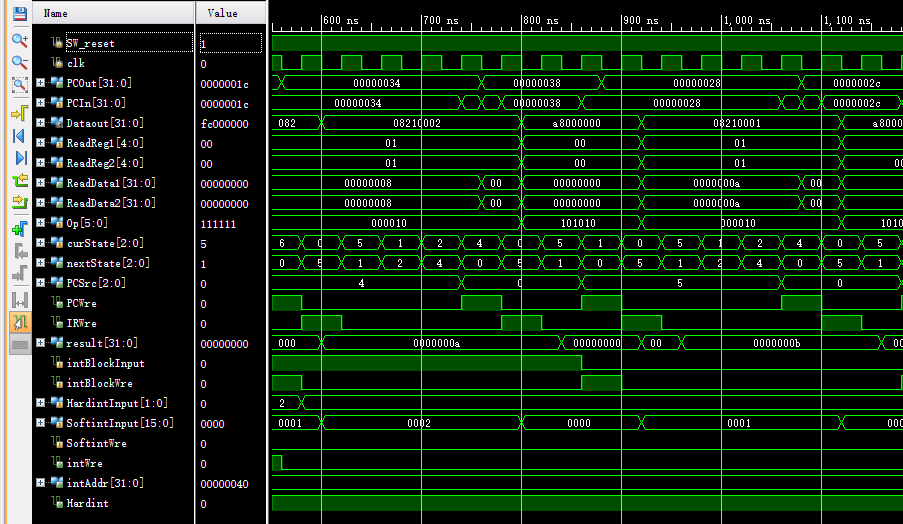
\includegraphics[scale=0.48]{../pics/img_2.png}
\end{figure}

\newpage

\begin{figure}[!h]
\centering
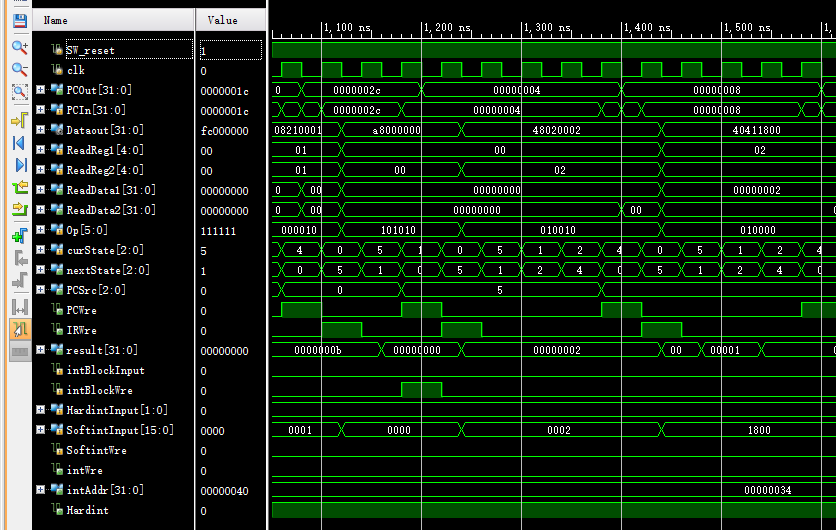
\includegraphics[scale=0.49]{../pics/img_3.png}
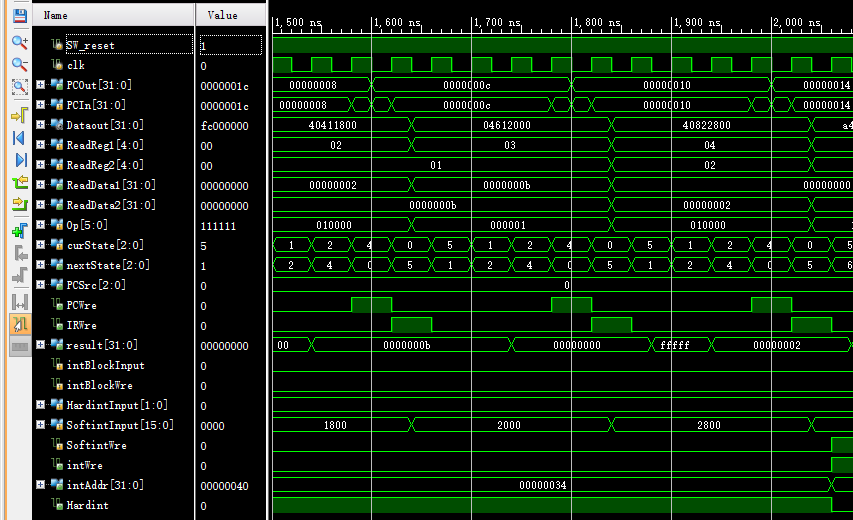
\includegraphics[scale=0.48]{../pics/img_4.png}
\end{figure}

\newpage

\begin{figure}[!h]
\centering
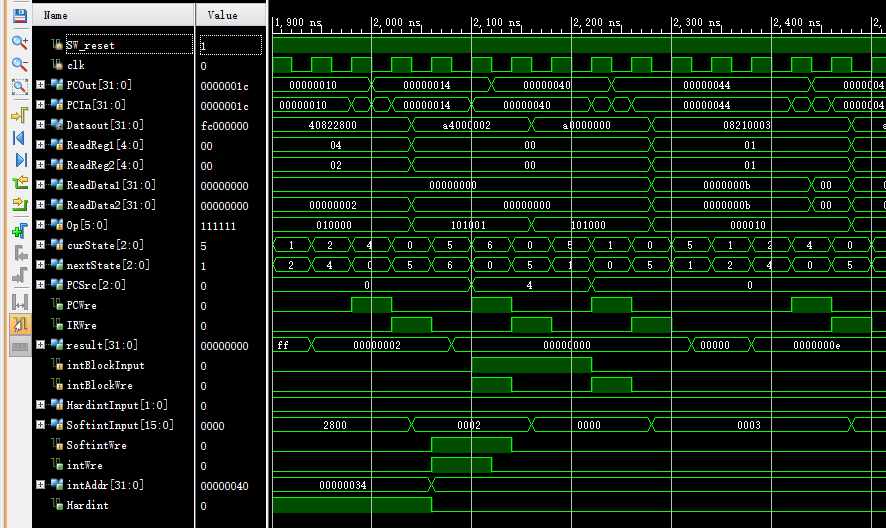
\includegraphics[scale=0.49]{../pics/img_5.png}
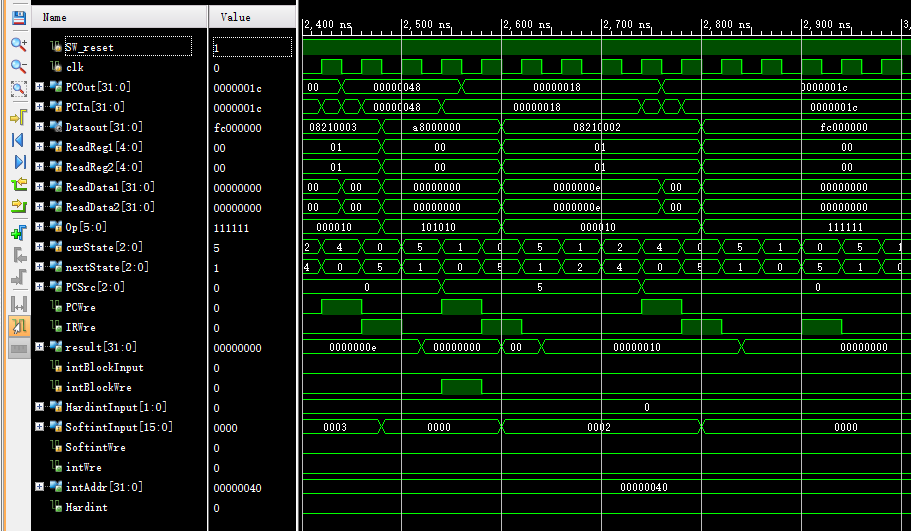
\includegraphics[scale=0.47]{../pics/img_6.png}
\end{figure}

\newpage

\section{中断控制器实现代码}

中断控制器是使用 Verilog 实现的。

为了实现简单,中断控制器里包含了中断向量存储器。

\begin{lstlisting}[language=verilog]
`timescale 1ns / 1ps

module InterruptControllor(
    input clk,
    input intBlockInput,
    input intBlockWre,
    input [1:0] HardintInput,
    input [15:0] SoftintInput,
    input SoftintWre,
    output reg intWre,
    output reg [31:0] intAddr,
    output reg Hardint
    );
    
    reg [7:0] rom[199:0];
    reg valid;
    initial begin
        $readmemb("./interrupt_vector.txt", rom);
        valid = 1;
    end
    always @ (negedge clk) begin
        if (intBlockWre) begin
            valid <= !intBlockInput;
        end
    end
    always @ (valid or intBlockInput or intBlockWre or HardintInput or SoftintInput or SoftintWre) begin
        if (!valid) begin
            intWre = 0;
        end else begin
            if (HardintInput[0]) begin
                intAddr[31:24] = rom[0];
                intAddr[23:16] = rom[1];
                intAddr[15:8] = rom[2];
                intAddr[7:0] = rom[3];
                intWre = 1;
                Hardint = 1;
            end else
            if (HardintInput[1]) begin
                intAddr[31:24] = rom[4];
                intAddr[23:16] = rom[5];
                intAddr[15:8] = rom[6];
                intAddr[7:0] = rom[7];
                intWre = 1;
                Hardint = 1;
            end else
            if (SoftintWre) begin
                intAddr[31:24] = rom[SoftintInput * 4];
                intAddr[23:16] = rom[SoftintInput * 4 + 1];
                intAddr[15:8] = rom[SoftintInput * 4 + 2];
                intAddr[7:0] = rom[SoftintInput * 4 + 3];
                intWre = 1;
                Hardint = 0;
            end else 
            begin
                intWre = 0;
            end
        end
    end
endmodule
\end{lstlisting}

\newpage

\section{硬件堆栈实现代码}

硬件堆栈是使用 Verilog 实现的。

\begin{lstlisting}[language=verilog]
`timescale 1ns / 1ps

module PCStack(
    input clk,
    input push,
    input pop,
    input [31:0] dataIn,
    output [31:0] dataOut
    );
    reg [31:0] stk[199:0];
    reg top;
    
    initial begin
        top = -1;
    end
    assign dataOut = (top < 0) ? 32'hz : stk[top];
    always @ (negedge clk) begin
        if (push && !pop) begin
            top = top + 1;
            stk[top] = dataIn;
        end else
        if (!push && pop) begin
            top = top - 1;
        end
    end
endmodule
\end{lstlisting}

\end{appendices}


\end{document}
















